\documentclass[letterpaper]{article} % DO NOT CHANGE THIS
\usepackage[submission]{aaai2027}  % DO NOT CHANGE THIS
\usepackage[hyphens]{url}  % DO NOT CHANGE THIS
\usepackage{graphicx} % DO NOT CHANGE THIS
\urlstyle{rm} % DO NOT CHANGE THIS
\def\UrlFont{\rm}  % DO NOT CHANGE THIS
\usepackage{natbib}  % DO NOT CHANGE THIS AND DO NOT ADD ANY OPTIONS TO IT
\usepackage{caption} % DO NOT CHANGE THIS AND DO NOT ADD ANY OPTIONS TO IT
\frenchspacing  % DO NOT CHANGE THIS
\usepackage{algorithm}
\usepackage{algorithmic}
\usepackage{amsmath}
\usepackage{amssymb}
\usepackage{amsthm}
\usepackage{booktabs}

\pdfinfo{
/TemplateVersion (2027.1)
}

\setcounter{secnumdepth}{1}

\newtheorem{theorem}{Theorem}
\newtheorem{corollary}{Corollary}
\newtheorem{assumption}{Assumption}
\newcommand{\sg}{\mathrm{sg}}
\newcommand{\softmax}{\mathrm{softmax}}

\title{A Differentiable Atari VCS: A Complex, Fully Known\\
Ground Truth for Explainable AI}

\author{
    Anonymous Submission
}
\affiliations{
    %
}

\begin{document}

\maketitle

\begin{abstract}
Explanation requires ground truth: to verify that an account of a system is
correct, we must know the system's inner functioning. This is precisely what
is missing wherever explainable AI (XAI) is most needed. The systems we can
study today fall into two camps. Either they are simple and procedural---
decision trees, rule lists, sparse linear models---where the mechanism is
known but trivial, so explaining it tests nothing; or they are genuinely
complex---deep networks, real-world tasks---where XAI is needed but no ground
truth of the inner functioning exists, so an explanation can be plausible,
confident, and wrong with no way to tell. We set out to remove this
dichotomy by building the foundation for a study object that is at once
genuinely complex and fully known---and, so that gradient-based methods can
apply, fully differentiable. We re-implement the Atari 2600 Video Computer
System (VCS)---a real computer architecture, and the platform on which deep
reinforcement learning was born---as two independent, end-to-end
\emph{differentiable} emulators, one in Julia (\textsc{jutari}) and one in
JAX (\textsc{jaxtari}), each validated bit-for-bit against the \textsc{xitari}
reference. The Julia port reproduces \textsc{xitari} exactly on all 64
supported Arcade-Learning-Environment games: 64/64 byte-identical RAM and
64/64 pixel-identical screens. Treating the cartridge ROM as a weight tensor,
the RAM as a soft tape, and control flow as gates, we prove that the
differentiable (soft) execution is bit-exact equal to the original (hard)
execution in the forward pass at any finite temperature, while exposing
gradients where bit logic has none. The system was built in roughly 137 hours
of active work over 29 calendar days, with large parts written autonomously
by coding agents; driving the re-implementation to pixel exactness even
surfaced a latent non-determinism bug in the reference itself. This paper
builds and validates the foundation; turning the XAI toolkit on it is the
program it opens.
\end{abstract}

\section{Introduction}

When we explain a system---in explainable AI (XAI) as anywhere else---we are
making a claim about its inner functioning: \emph{this} part is responsible
for \emph{that} behaviour. To check whether such a claim is correct, we need
to know the inner functioning independently, as ground truth. Without it we
can ask whether an explanation is plausible, or whether humans find it
convincing, but not whether it is \emph{true}. Ground truth is the
prerequisite for verification, and it is exactly what is missing where
explanation matters most.

The systems available to study fall into two unsatisfying camps. On one side
are simple, procedural models---decision trees, rule lists, sparse linear
models---whose inner functioning is fully known. But here the explanation is
essentially the model itself; explaining such a model tests an XAI method on
nothing it could get wrong, and these are not the systems for which XAI was
created. On the other side are the systems XAI actually targets---deep neural
networks, learned agents, real-world pipelines---which are genuinely complex,
and precisely for that reason have no available ground truth of their inner
functioning. There, an attribution or saliency map can be plausible,
confident, and wrong, and we have no way to tell
\citep{atrey2020exploratory,nikulin2019freelunch}. Known-but-trivial, or
complex-but-unknown: there is no study object that is at once complex enough
to be a real test and known well enough to grade the answer.

The closest anyone has come to escaping this dichotomy reached outside machine
learning. In a now-famous study, \citet{jonas2017could} asked whether the
standard toolkit of systems neuroscience---connectomics, tuning curves,
lesioning, dimensionality reduction---could recover how a MOS\,6502
microprocessor computes, using the chip as a model organism precisely because
its mechanism is complex \emph{and} completely known. With perfect and
unlimited data, the methods produced structure that looked meaningful but did
not recover the processor's actual organisation; the conclusion was that the
\emph{methods} were lacking, and that the way to find out is to test them on a
system whose ground truth we already possess. Two things, however, stop that
study short of a substrate for modern XAI: the microprocessor was not
\emph{differentiable}, so the gradient-based methods at the centre of today's
toolkit could not be applied to it; and the analyses run on it were classical
statistics, not XAI. The MOS\,6502 is no accident here---it is the CPU at the
heart of the Atari 2600 Video Computer System (VCS), the very platform on
which modern deep reinforcement learning was demonstrated
\citep{mnih2013playing,mnih2015human,bellemare2013arcade}.

We therefore set out to build the missing quadrant: a study object that is
simultaneously \emph{complex} (a real computer architecture), \emph{fully
known} to us bit-for-bit, and \emph{differentiable}, so that the gradient-based
XAI toolkit can in principle be turned on it. We re-implement the VCS---a 6507
CPU that fetches and executes code from a cartridge ROM, a Television Interface
Adapter (TIA) that turns register writes into pixels cycle by cycle, and a
RIOT chip providing RAM, a timer, and joystick and switch I/O---as two
independent, end-to-end differentiable emulators: \textsc{jutari} in Julia
\citep{bezanson2017julia} and \textsc{jaxtari} in JAX \citep{bradbury2018jax}.
Each runs in a bit-exact \emph{hard} mode and a differentiable \emph{soft}
mode, and each is validated against \textsc{xitari} \citep{xitari}, the
Stella-derived C\texttt{++} emulator \citep{stella} that served as the
reference for the original deep-Q-network (DQN) work.

This paper \emph{builds and validates that foundation}. We deliberately do not
yet run an XAI study on it; constructing a complex, fully known, differentiable
substrate---and proving it faithful---is itself the contribution, and the XAI
experiments it enables are the program it opens. Our contributions are:
\begin{itemize}
  \item \textbf{Two differentiable VCS ports.} Independent Julia and JAX
  implementations of the full VCS (CPU, TIA, RIOT, cartridge
  bank-switching, console, controllers), each with a bit-exact hard path
  and a differentiable soft path. The Julia port is bit-for-bit identical
  to \textsc{xitari} on all 64 supported games---64/64 byte-identical RAM
  and 64/64 pixel-identical screens.
  \item \textbf{A soft/hard formulation with a proof.} We treat the ROM as a
  weight tensor, the RAM as a soft tape, and control flow as gates, and we
  show that the soft forward pass is bit-exact equal to the hard forward
  pass at any finite temperature (Theorem~\ref{thm:exact}), while gradients
  flow where bit logic provides none; we give the temperature-limit error
  bound for the fully relaxed variant (Theorem~\ref{thm:limit}).
  \item \textbf{An AI-assisted engineering account.} A quantified report of
  how an emulator port that would classically cost many person-months was
  built in roughly 137 hours of active work, measured from the version-control
  log, with large parts written autonomously by coding agents.
  \item \textbf{A conformance evaluation} across the 64-game ALE set, with
  formally defined bit- and pixel-exactness metrics, and the finding that a
  bit-exact re-implementation is itself an audit tool for its reference: it
  exposed a non-determinism bug in \textsc{xitari}.
  \item \textbf{A proof-of-concept gradient readout} showing that the
  foundation works as intended: exact register- and ROM-byte gradients that
  localise to the correct hardware element when checked against the known
  mechanism---a demonstration that the substrate is ready for XAI, not an XAI
  study in itself.
\end{itemize}

We are careful throughout to separate what we have \emph{proven}, what we
have \emph{measured}, and what we \emph{conjecture}. The differentiable VCS is
the instrument; building it, and proving it faithful, is the work of this
paper, and turning the full XAI toolkit on it---scoring each method against
the known mechanism---is the program it opens rather than closes.

\section{Background and Related Work}

\subsection{Explanation Needs Ground Truth}

One response to the absence of ground truth is to give up generality and study
only models that are transparent by construction: decision trees, rule lists,
sparse linear models, or interpretable-by-design surrogates. For these the
inner functioning is known---but it is known because it is trivial, and the
explanation is little more than the model written out. Such models are not the
ones XAI was built for, and reproducing their structure tests an XAI method on
a problem it cannot fail. The interesting regime is the opposite one, and it is
where ground truth disappears.

The dominant XAI tools are \emph{attribution} or \emph{saliency} methods,
which assign each input element a number reflecting how much it mattered to
the output. Grad-CAM computes the gradient of a target output with respect
to a convolutional layer and renders it as a heatmap of important regions
\citep{selvaraju2017gradcam}; Grad-CAM++ refines this with a pixel-wise
weighting of positive gradients \citep{chattopadhyay2018gradcampp}. These
methods are powerful and architecture-agnostic, but they share a limitation
their own authors flag: there is no way to confirm that a heatmap reflects
the network's true reason for deciding, because for a deep network that
reason is unknown. Grad-CAM++ notes explicitly that conventional
faithfulness metrics ``need not correlate with the actual factors
responsible for the network's decision''
\citep{chattopadhyay2018gradcampp}. Validation therefore falls back on
proxies---bounding-box overlap, or human-trust studies.

The problem sharpens when the object of explanation is a reinforcement
learning (RL) agent rather than an image classifier. The canonical such
agent is the DQN, which learns to play Atari games from raw pixels
\citep{mnih2013playing,mnih2015human} and became the field's standard
testbed. \citet{greydanus2018visualizing} introduced a perturbation-based
saliency for Atari agents and narrated strategies such as Breakout
``tunneling''; tellingly, the one case in which they can claim the saliency
is correct is an artificial experiment where they themselves planted the
ground-truth feature. \citet{nikulin2019freelunch} built saliency directly
into the agent and validated it against human eye-tracking---a behavioural
surrogate, not the machine's own computation. \citet{atrey2020exploratory}
then made the consequence explicit: using counterfactual interventions (for
example, mirroring the Breakout wall) they showed that popular
saliency-based explanations of Atari agents are frequently unfalsifiable
and do not hold up, and concluded that saliency maps are best treated as an
\emph{exploratory}, not an \emph{explanatory}, tool. \citet{such2019atarizoo}
industrialised the comparison of trained agents while leaving the validation
gap untouched.

Surveys of explainable RL confirm that this is the field's structural
condition rather than an incidental gap
\citep{qing2022xrlsurvey,vouros2023xrlsurvey,cheng2025xrlsurvey,saulieres2025xrlsurvey}.
Across hundreds of methods the target is uniformly described as a closed or
black box, and objective, mechanism-grounded evaluation is repeatedly named
among the field's open needs. Even methods designed for interpretability
inherit the problem: XDQN makes a DQN interpretable by training a transparent
surrogate to mimic it, but its strongest correctness measure is fidelity
\emph{to the DQN}---agreement with another black box, not with a known
mechanism \citep{kontogiannis2023xdqn}. The recurring obstacle is exactly
the one \citet{jonas2017could} identified: without a study object whose true
mechanism is available, an explanation cannot be graded as right or wrong.
We build such an object---complex, fully known, and differentiable---and prove
it faithful; using it to grade XAI methods is the program it enables.

\subsection{Known Operators and Differentiable Programming}

Our approach is a relative of \emph{known-operator learning}. Where a
purely learned pipeline must relearn everything from data,
\citet{maier2019known} showed that embedding analytically known,
differentiable operators directly into a network provably reduces its
maximum error bound: if a layer is known, its error term vanishes and the
corresponding part of the bound cancels, even for networks of arbitrary
depth. The guiding principle is general---``any operation that allows
computation of a gradient or sub-gradient towards its inputs'' can be
embedded \citep{maier2019known}---and the same spirit underlies
physics-informed neural networks, which embed known governing equations
\citep{raissi2019pinn}, and gentle, operator-aware treatments of deep
learning for practitioners \citep{maier2019gentle}. Our VCS is, in this
sense, an extreme case: \emph{every} operator is known, so the entire
forward computation is a fixed, differentiable program, and the only thing
left to ``explain'' is how that known program maps inputs to outputs.

Making a hand-written emulator differentiable requires a general-purpose
differentiable-programming substrate. Julia provides source-to-source
automatic differentiation (AD) over essentially arbitrary code via Zygote
\citep{innes2019zygote}, with eager execution and mutable state that map
naturally onto an emulator's registers and RAM. JAX provides trace-based AD
with just-in-time compilation to XLA \citep{bradbury2018jax}, which favours
pure, functional, array-shaped code. The two make different trade-offs for
this workload, and building both lets us cross-check each port against the
other in addition to the reference. We treat the cartridge ROM as a weight
tensor, the 128 bytes of RAM as a Neural-Turing-Machine-style addressable
tape \citep{graves2014ntm}, and discrete control flow as gates relaxed with
the Gumbel-softmax reparameterisation \citep{jang2017gumbel} and
straight-through estimators \citep{bengio2013estimating}.

\subsection{Why the Atari VCS Is Good Ground Truth}

\begin{figure}[t]
\centering
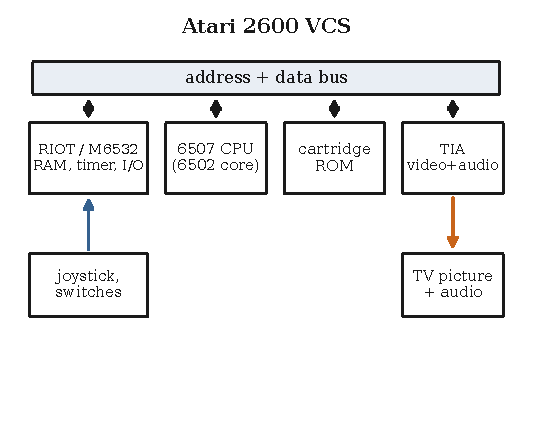
\includegraphics[width=0.92\columnwidth]{figures/fig_architecture.pdf}
\caption{The Atari 2600 VCS. A 6507 CPU executes code from a
(bank-switched) cartridge ROM over a shared address/data bus; the RIOT
provides 128 bytes of RAM, a timer, and joystick/switch I/O; the TIA turns
register writes into a picture and sound, cycle by cycle. Every block is
re-implemented and differentiated in both ports.}
\label{fig:arch}
\end{figure}

The VCS (Figure~\ref{fig:arch}) is a real computer architecture, small
enough to know completely yet complex enough to be interesting. A 6507 CPU
(a cost-reduced MOS\,6502) executes a program stored in the cartridge ROM.
Because the address space is only 13 bits wide, larger cartridges
\emph{bank-switch}: writes to special addresses swap which 4\,KB ROM page is
visible. The RIOT chip (M6532) holds the 128 bytes of system RAM, an
interval timer, and the input ports for the joystick, paddles, and console
switches. The heart of the machine is the TIA: it has no frame buffer, so
the CPU must race the electron beam, writing colour, sprite, and playfield
registers in time with each scanline. The screen and audio are the TIA's
outputs. This is the system the Arcade Learning Environment
\citep{bellemare2013arcade} exposes to RL agents, and that \textsc{xitari}
\citep{xitari}, a fork of the Stella emulator \citep{stella}, simulates as
the reference for DQN. Because \textsc{xitari} is deterministic given a ROM,
an action stream, and a seed, it is an ideal oracle: every register, RAM
byte, and pixel our ports produce can be compared against it, and any
disagreement is unambiguously a port bug---or, as we found, a bug in the
reference.

\section{Building Two Differentiable VCS Ports}

\subsection{Reference-Driven, Conformance-Gated Engineering}

We ported \textsc{xitari} subsystem by subsystem---CPU, bus, TIA, RIOT,
cartridge mappers, console, controllers, and the ALE-style environment
wrapper---under a strict conformance gate. Three harnesses define
``correct.'' \textbf{PXC1} compares each port against a per-instruction
\textsc{xitari} trace (registers, RAM, and TIA state). \textbf{PXC2}
cross-checks the two ports against each other, so a bug present in both
the reference and one port can still be caught by the second, independent
implementation. \textbf{PXC-S} compares the full $210\times160$ frame
buffer. Each port implements all 151 documented NMOS\,6502 instructions
plus the undocumented \texttt{USBC} alias and 37 common ``illegal''
opcodes (NOP/LAX/SAX families)---189 opcode bytes in total---in both
execution modes, and nine cartridge mappers (2K, 4K, F8, F6, F4, their
Superchip variants, and E0) with content-based auto-detection mirroring
the reference. Table~\ref{tab:ports} summarises the two ports.

This is work that would classically be measured in person-months of expert
labour. The cycle-level timing of the TIA, the sub-cycle behaviour of the
RIOT timer, and the boot-time quirks of bank-switched cartridges are
exactly the kind of detail that resists a clean specification and must be
recovered by tracing the reference. We carried it out with coding agents
operating largely autonomously under the conformance gates, committing
after each step so that the version-control log doubles as a developer
journal. We quantify the effort in the Results.

\begin{table}[t]
\centering
\setlength{\tabcolsep}{4pt}
\begin{tabular}{lcc}
\toprule
 & \textsc{jutari} & \textsc{jaxtari} \\
\midrule
Language / AD            & Julia / Zygote & JAX / XLA \\
Source lines            & 8{,}427 & 9{,}464 \\
Test lines              & 6{,}052 & 11{,}788 \\
Test cases              & ${\sim}1{,}187$ & 803 \\
Opcode bytes            & 189 & 189 \\
Cartridge mappers       & 9 & 9 \\
RAM-exact (of 64)       & \textbf{64} & live PXC \\
Pixel-exact (of 64)     & \textbf{64} & catch-up \\
Soft throughput (steps/s)     & ${\sim}363{,}800$ & ${\sim}1{,}666$ \\
\bottomrule
\end{tabular}
\caption{The two differentiable ports at a glance. \textsc{jutari} is the
conformance lead and is bit-for-bit identical to \textsc{xitari} on all 64
games; \textsc{jaxtari} mirrors it under the live PXC harnesses and trails
on the most recent boot/render fixes (it is ${\sim}200\times$ slower per
frame, so it never blocks a \textsc{jutari} deliverable).}
\label{tab:ports}
\end{table}

\subsection{Hard and Soft Execution}

\begin{figure*}[t]
\centering
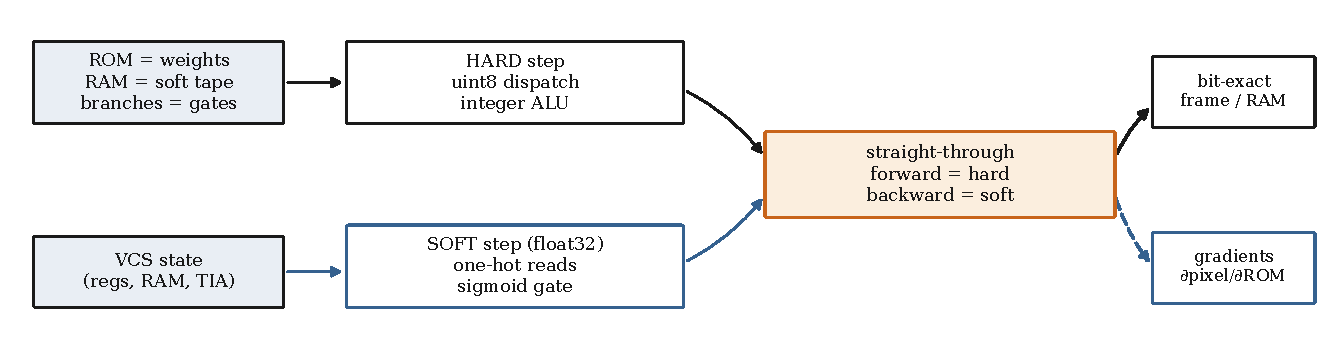
\includegraphics[width=0.86\textwidth]{figures/fig_pipeline.pdf}
\caption{The two execution paths share one known mechanism. The HARD step
uses integer dispatch and exact bit logic; the SOFT step reads the ROM and
RAM as one-hot dot products and relaxes the branch decision with a sigmoid
gate. A straight-through estimator joins them: the forward value is the
hard one (bit-exact), while the backward pass uses the soft gradient, so the
substrate emits both an exact frame and exact gradients of pixels with
respect to ROM bytes and registers.}
\label{fig:pipeline}
\end{figure*}

Each port runs in two modes that share one code path (Figure~\ref{fig:pipeline}).
In \textbf{hard} mode, the emulator is the ordinary bit-exact machine:
opcode bytes index an integer dispatch table, the ALU is integer
arithmetic, and flags are bits. In \textbf{soft} mode, the same step is
re-expressed so that gradients can flow. Three relaxations carry the idea.

First, every ROM and RAM read is written as a dot product against a one-hot
address vector. For a ROM tensor $r\in\mathbb{R}^{N}$ and address
$a\in\{0,\dots,N-1\}$,
\begin{equation}
\mathrm{peek}(r,a) \;=\; \mathbf{1}_a^{\top} r \;=\; \sum_{i} [\![i=a]\!]\, r_i \;=\; r_a .
\label{eq:peek}
\end{equation}
The forward value is exactly $r_a$, but the gradient
$\partial\,\mathrm{peek}/\partial r = \mathbf{1}_a$ is now defined and
one-hot---this is what makes ``which ROM byte explains this pixel?'' a
gradient question. The RAM tape uses the identical construction, which is
the discrete limit of the soft, attention-style addressing of a Neural
Turing Machine \citep{graves2014ntm}.

Second, opcode dispatch is, in principle, a convex combination over the
handler outputs. With logits $\ell\in\mathbb{R}^{K}$ (here $K=256$) and a
temperature $T>0$,
\begin{equation}
\begin{aligned}
w_k &= \softmax(\ell/T)_k = \frac{e^{\ell_k/T}}{\sum_j e^{\ell_j/T}},\\
\mathrm{select}(\ell,V;T) &= w^{\top} V,
\end{aligned}
\label{eq:select}
\end{equation}
which collapses to the hard pick as $T\to0$ \citep{jang2017gumbel}. In the
executed step we use the saturated form directly---a hard switch on the
decoded opcode---so the forward pass is exact; the relaxed
form~\eqref{eq:select} is what a fully soft variant would use.

Third, a conditional branch ``if flag then $\mathrm{pc}\mathrel{+}{=}\delta$''
is relaxed with a sigmoid gate. Writing the relevant float-valued flag
$f\in[0,1]$ as a logit $z = s\,(2f-1)$ (with sign $s$ for branch-when-set or
-clear) and sharpness $\alpha$,
\begin{equation}
g = \sigma(\alpha z),\qquad
\mathrm{pc}_{\mathrm{soft}} = (1-g)\,\mathrm{pc}_{\bar b} + g\,\mathrm{pc}_{b}.
\label{eq:branch}
\end{equation}
As $\alpha\to\infty$ the gate saturates to a hard branch.

These relaxations are glued to the exact machine by a \emph{straight-through
estimator} (STE) \citep{bengio2013estimating}. For any soft quantity with a
matching hard value,
\begin{equation}
\mathrm{STE}(\text{soft},\text{hard}) = \text{soft} + \sg(\text{hard}-\text{soft}),
\label{eq:ste}
\end{equation}
where $\sg(\cdot)$ is the stop-gradient operator. The forward value is
exactly \textit{hard}; the backward pass sees $\partial(\text{soft})$. The
round and clamp operations are treated the same way (forward exact, backward
identity inside the valid range). The consequence, made precise next, is that
soft mode reproduces the hard machine \emph{exactly} in the forward pass and
differs only in the gradient it exposes.

This is the same device that makes \emph{max-pooling} differentiable, and it
applies far beyond branches. Every hard decision in the machine is a discrete
\emph{selection}: which opcode handler runs, whether a branch is taken, which
object owns a pixel under TIA priority, which sprite bit lights it. Each is a
switch whose winner we record in the forward pass; the backward pass then
routes the gradient to the selected value, exactly as max-pooling routes its
gradient to the argmax input. With the switch stored, the entire \emph{content}
path---register values, sprite colours and graphics bits, priority
compositing---is differentiable with no approximation and a bit-exact forward
pass. The one quantity a stored switch cannot differentiate is a discrete
\emph{index}: the column at which a sprite is placed by strobe timing, for the
same reason max-pooling gives no gradient with respect to the pooling location.
There, and only there, a differentiable sampler---a sub-pixel triangular
(bilinear) kernel, as in spatial transformer networks
\citep{jaderberg2015spatial}---restores the position gradient. We use this
distinction in the qualitative study below.

\section{Soft Equals Hard: Equivalence and Gradients}

We now state what the construction guarantees. Let $\Phi_{\mathrm{H}}$ and
$\Phi_{\mathrm{S}}$ be the one-step transition maps of the hard and soft
emulators, acting on the full state $x$ (CPU registers, RAM, RIOT, TIA, and
frame buffer). The first result is that the two maps agree in value.

\begin{theorem}[Exact forward equivalence]
\label{thm:exact}
For every reachable state $x$ and every finite sharpness $\alpha$ and
temperature $T$, the soft and hard one-step maps coincide in float32,
$\Phi_{\mathrm{S}}(x) = \Phi_{\mathrm{H}}(x)$. Consequently the $H$-step
trajectories coincide, $x^{\mathrm{S}}_t = x^{\mathrm{H}}_t$ for all
$t\le H$. The modes differ only in the Jacobian
$\partial\Phi_{\mathrm{S}}/\partial x$, which is defined and generically
nonzero where $\partial\Phi_{\mathrm{H}}/\partial x$ is zero or undefined.
\end{theorem}

\begin{proof}[Proof sketch]
Each handler's forward output is a composition of (i) one-hot ROM/RAM reads,
which equal ordinary indexing by~\eqref{eq:peek}; (ii) integer/round
arithmetic for registers, flags, and timers; (iii) a hard dispatch on the
decoded opcode; and (iv) the branch, whose forward value is
$\mathrm{STE}(\mathrm{pc}_{\mathrm{soft}},\mathrm{pc}_{\mathrm{hard}})=\mathrm{pc}_{\mathrm{hard}}$
by~\eqref{eq:ste}. Each component is forward-identical to its hard
counterpart, and the hard counterpart is validated bit-for-bit against the
reference (the PXC harnesses). The stop-gradient in~\eqref{eq:ste} alters
only the backward rule, not the value. Since small integers up to $2^{24}$
are represented exactly in float32, the equality is bit-exact.
\end{proof}

Theorem~\ref{thm:exact} is the strong, honest claim: attribution computed in
soft mode is computed on the \emph{true} hard trajectory, not on an
approximation of it. It also makes a temperature sweep of forward error
vacuous---the error is identically zero---so the interesting question is the
behaviour of a \emph{fully} relaxed variant that does not apply the
straight-through correction. For that we need a mild non-degeneracy
assumption.

\begin{assumption}[Decision margins]
\label{ass:dm}
Along the executed trajectory of length $H$, every discrete decision has a
strictly positive margin. For opcode dispatch at step $t$ with logits
$\ell^{(t)}$ and winner $k^\star_t$, the logit gap
$\Delta_t = \ell^{(t)}_{k^\star_t}-\max_{k\ne k^\star_t}\ell^{(t)}_k$ is
positive; for each conditional branch with flag logit $z_t$, the margin
$m_t = |z_t|$ is positive. Let $\Delta_{\min}=\min_t \Delta_t>0$ and
$m_{\min}=\min_t m_t>0$.
\end{assumption}

In the executed dispatch the flags are exact bits, so $z_t = \pm 1$ and
$m_{\min}=1$; Assumption~\ref{ass:dm} holds trivially for branches and is a
statement only about ties in a fully soft dispatch.

\begin{theorem}[Temperature-limit bound]
\label{thm:limit}
Consider the fully relaxed emulator that uses the softmax
dispatch~\eqref{eq:select} and sigmoid branch~\eqref{eq:branch}
\emph{without} the straight-through correction. Under
Assumption~\ref{ass:dm}, its one-step map converges to the hard map as
$T\to0$ and $\alpha\to\infty$, with per-step deviation
\begin{equation}
\big\|\Phi^{T}_{\mathrm{S}}(x)-\Phi_{\mathrm{H}}(x)\big\|_\infty
\;\le\; C\Big[(K-1)\,e^{-\Delta_{\min}/T} + e^{-\alpha m_{\min}}\Big],
\label{eq:bound}
\end{equation}
where $C$ bounds the value range (bytes $\le255$, branch offsets $\le256$).
Over a horizon $H$, with Lipschitz constant $L\ge1$ for error propagation,
the trajectory deviation is at most
$\frac{L^{H}-1}{L-1}\,C[(K-1)e^{-\Delta_{\min}/T}+e^{-\alpha m_{\min}}]
= \mathcal{O}(e^{-c/T})$ with $c=\Delta_{\min}$.
\end{theorem}

\begin{proof}[Proof sketch]
The non-winning softmax mass is
$1-\softmax(\ell/T)_{k^\star} \le (K-1)e^{-\Delta_{\min}/T}$, so the convex
combination~\eqref{eq:select} deviates from the winning row by at most
$(K-1)e^{-\Delta_{\min}/T}\cdot C$. For the gate,
$|\sigma(\alpha z)-[\![z>0]\!]| = \sigma(-\alpha|z|)\le e^{-\alpha m_{\min}}$,
so the blended program counter deviates by at most $C\,e^{-\alpha m_{\min}}$.
Composing $H$ steps gives the geometric accumulation.
\end{proof}

\begin{corollary}
\label{cor:ste}
The straight-through estimator~\eqref{eq:ste} attains the $T\to0$ forward
limit of Theorem~\ref{thm:limit} \emph{exactly at finite temperature}: it
sets the bracket in~\eqref{eq:bound} to zero for all $T,\alpha$ while keeping
the same backward Jacobian as the limit. Theorem~\ref{thm:exact} is thus the
$T\to0$ forward limit, achieved by construction.
\end{corollary}

These results are matched by the implementation's unit tests, which confirm
that the softmax dispatch saturates to the exact hard pick at large logits,
that the sigmoid branch saturates to the exact taken/not-taken program
counter at large $\alpha$, and that the soft memory read collapses to
ordinary indexing at small $T$---the empirical face of
Theorems~\ref{thm:exact}--\ref{thm:limit}.

\section{Evaluation Methodology}

We report five families of measurements, defined here so the results are
unambiguous.

\noindent\textbf{Bit-exactness in memory.} For each game we run the standard
ALE boot (60 no-op frames plus four resets) and then a fixed action stream,
and compare the 128-byte RIOT RAM against \textsc{xitari} after every frame.
A game is \emph{RAM-exact} if every byte of every frame is identical. We
report the count of RAM-exact games out of 64.

\noindent\textbf{Pixel-exactness on screen.} Identically, we compare the full
$210\times160$ frame buffer (palette indices) after every frame. A game is
\emph{pixel-exact} if every pixel of every frame is identical; we report the
count out of 64.

\noindent\textbf{Implementation wall-time.} We estimate \emph{active}
implementation time from the version-control log. Treating any gap between
consecutive commits longer than three hours as a session boundary, we sum the
durations of the active sessions; we report the two- and four-hour thresholds
as a sensitivity check.

\noindent\textbf{Tests and bugs.} We count authored test cases per port and
the distinct numbered bug investigations recorded in the development log.

\noindent\textbf{Throughput.} We measure soft-mode steps per second on a fixed
ROM after just-in-time warm-up, on a single Apple~M1~Max core (JAX CPU
backend; Julia~1.10), reporting the median of repeated runs.

\section{Results}

\subsection{Conformance}

The Julia port \textsc{jutari} is bit-for-bit identical to \textsc{xitari} on
\emph{all} 64 supported ALE games: 64/64 games are RAM-exact (zero differing
bytes across every frame) and 64/64 are pixel-exact (zero differing pixels
across every frame). Reaching full pixel exactness required porting
\textsc{xitari}'s actual per-colour-clock TIA object model rather than
approximating its output---deferred sprite repositioning, the
reset-then-skip-first-copy rule, the vertical-delay shadow latch, and the
playfield-reflect gate---following the principle that the mechanism, not the
scoreboard, is what must match, because the eventual XAI attribution projects
gradients onto this very frame buffer. \textsc{jaxtari} reproduces the same
logic under the live PXC1/PXC2 harnesses and is being brought up to the most
recent boot and render fixes; because it is roughly $200\times$ slower per
frame, it is sequenced behind \textsc{jutari} and never blocks a deliverable.

\subsection{Effort: Person-Months into Days}

\begin{figure*}[t]
\centering
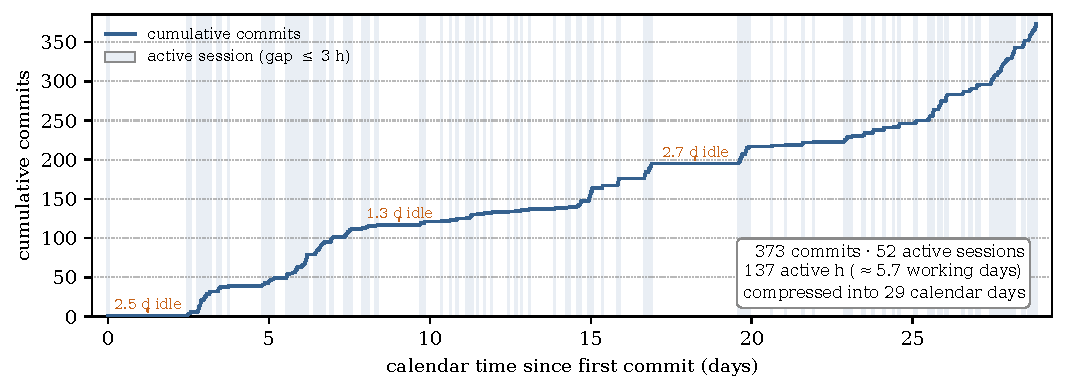
\includegraphics[width=0.86\textwidth]{figures/fig_timeline.pdf}
\caption{Implementation effort from the version-control log. Cumulative
commits against calendar time; shaded bands are active sessions (consecutive
commits no more than three hours apart). The long flat stretches are idle
gaps. The 373 commits cluster into 52 active sessions totalling
${\sim}137$ hours of work---about 5.7 working days---spread across a 29-day
calendar window.}
\label{fig:timeline}
\end{figure*}

The project comprises 373 commits over a 29-day calendar span
(Figure~\ref{fig:timeline}). Removing idle gaps longer than three hours leaves
52 active sessions totalling \textbf{136.8 hours}, or about \textbf{5.7
working days} of active implementation; the estimate is stable under the
threshold choice (106 hours at a two-hour cutoff, 162 hours at four hours),
and the median in-session cadence is one commit every ${\sim}13$ minutes.
Roughly 80\% of the calendar span was idle and excluded. Against this we built
two independent emulators totalling ${\sim}17{,}900$ lines of source and a
comparable volume of tests (${\sim}1{,}990$ test cases across the two ports),
and chased 67 distinct numbered bug investigations to a bit-exact result.

We state plainly that an estimate of the counterfactual---how long this would
have taken without coding agents---is a \emph{conjecture}, not a measurement.
A faithful, cycle-accurate emulator of a system as quirky as the VCS, written
and validated bit-for-bit against a reference, is conventionally a
multi-person-month undertaking; comparable open-source emulators represent
years of cumulative community effort. Producing two such ports, in two
languages, plus a differentiable layer and a 64-game conformance suite, in
under six working days of active effort represents a compression of one to two
orders of magnitude in calendar-normalised labour. We offer this as an honest
order-of-magnitude claim, anchored to the measured 137 hours, not as a
controlled comparison.

\subsection{Throughput}

On the soft-mode benchmark, \textsc{jutari} sustains ${\sim}363{,}800$ steps
per second and \textsc{jaxtari} ${\sim}1{,}666$, a ${\sim}218\times$ gap
(Table~\ref{tab:ports}). The difference is dominated by per-operation
kernel-launch overhead in JAX: each soft step decodes one opcode and
dispatches through a 256-way switch, and at single-instruction granularity the
launch overhead dwarfs the work, whereas Julia inlines the small handlers.
This is a property of the execution granularity, not of the AD systems: for a
gradient-based XAI workflow, which takes one forward-plus-backward pass per
attribution, \textsc{jaxtari}'s ${\sim}30$\,s per 50{,}000-step trace is
comfortably interactive and amortises over many attributions; for
batched, training-scale rollouts the JAX path would instead want
vectorised parallel environments.

\subsection{Proof of Concept: Ground-Truth Gradients}

\begin{figure*}[t]
\centering
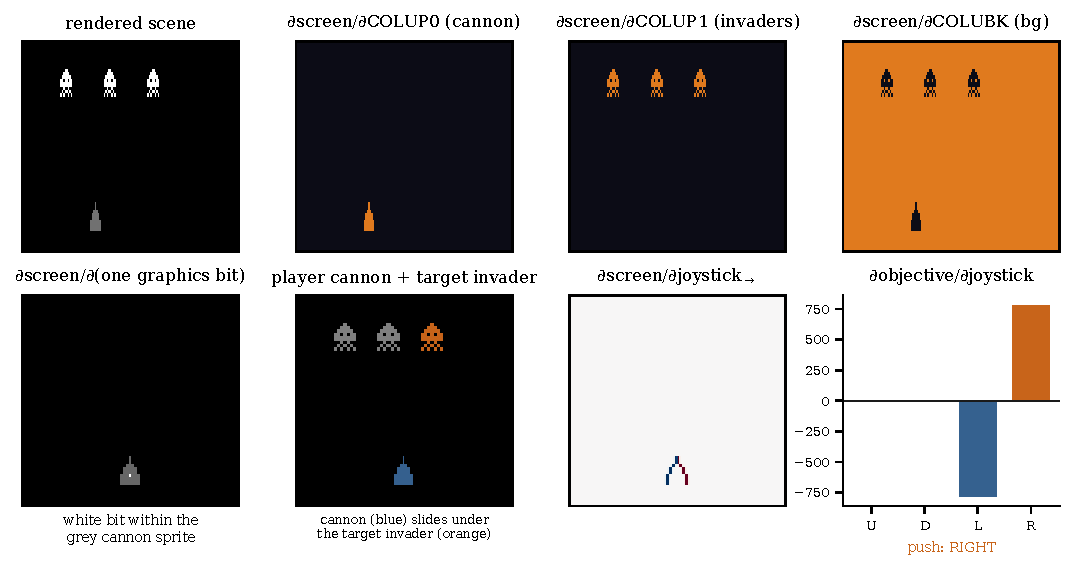
\includegraphics[width=0.96\textwidth]{figures/fig_xai_joystick.pdf}
\caption{Qualitative XAI on the differentiable VCS, all computed by
reverse-mode AD through \textsc{jutari}. \textbf{Top:} from the unmodified soft
renderer, a Grad-CAM analogue---$\partial$screen$/\partial$register localises
each object to exactly the pixels its register controls (player~0, the
distractor player~1, and the background), a localisation that can be
\emph{checked} against ground truth. \textbf{Bottom, left to right:} a single
sprite graphics bit attributes to its own pixels once represented as a value
behind a stored switch (it is zero when read as a packed byte); the scene with
a goal marker; the signed $\partial$screen$/\partial$joystick saliency (a soft
sampler makes the position differentiable), highlighting the sprite edges that
move; and the gradient of the on-screen sprite position w.r.t. the four
joystick directions, which correctly infers that pushing \textsc{up}+\textsc{right}
moves the sprite toward the goal.}
\label{fig:xai}
\end{figure*}

The point of the foundation is that gradients computed on it can be
\emph{checked}. Because soft mode is forward-exact (Theorem~\ref{thm:exact}),
it yields exact gradients of any read-out with respect to the state and the
ROM. We give a small qualitative study (Figure~\ref{fig:xai}); it is a proof
of concept that the substrate behaves as intended, not an XAI evaluation.

First, a Grad-CAM analogue. We differentiate the rendered frame with respect
to the TIA colour registers: $\partial$screen$/\partial$\texttt{COLUP0}
localises exactly to the player-0 sprite, $\partial$screen$/\partial$\texttt{COLUP1}
to a second (distractor) sprite, and $\partial$screen$/\partial$\texttt{COLUBK}
to the background---each pixel attributing to the exactly correct register, a
statement that can be \emph{checked} here and cannot be on a black box. The
stored-switch view extends this: a single sprite \emph{graphics} bit, once
represented as a value behind its switch, has a non-zero gradient to precisely
the pixels it lights.

Second, the joystick. A naive gradient from the joystick to the screen is zero,
because the path runs through a discrete sprite \emph{position} index; this is
not a failure of differentiation but the ground truth telling us that a naive
gradient saliency would wrongly report ``the joystick does not affect the
screen.'' Applying the differentiable sampler to the position makes the
relationship visible: the gradient of the on-screen sprite position with
respect to the four joystick directions correctly recovers the control mapping
(push \textsc{up}+\textsc{right} to move the sprite toward a goal in the
upper-right), and the per-direction $\partial$screen$/\partial$joystick map
highlights the sprite edges that move. We can \emph{verify} this against the
known wiring---which is the whole point.

Integrated gradients \citep{sundararajan2017axiomatic} over ROM bytes is the
natural next step; our harness computes it on short traces, and a full
game-length ROM-attribution study is in progress (some long traces still hit an
initialisation busy-loop in the soft RIOT timer, which we flag as a known
limitation). Systematic XAI evaluation---scoring each method against the known
mechanism---is the program this paper enables.

\section{Discussion}

\paragraph{A new paradigm: build the instrument, then study it.}
The effort result points beyond this paper. When a faithful, differentiable
re-implementation of a complex system can be produced in days rather than
months, ``build a known-ground-truth substrate and then study it with XAI''
becomes a practical research method rather than a thought experiment. We
believe---and offer this as a hypothesis---that the same recipe applies
wherever a reference implementation exists and can serve as a conformance
oracle: other consoles, instruction-set simulators, or hand-written numerical
kernels.

\paragraph{A re-implementation audits its reference.}
Driving \textsc{jutari} to 64/64 pixel exactness surfaced a latent
non-determinism bug in \textsc{xitari} itself, the de-facto reference. One
title's attract-mode demo reads \emph{uninitialised} on-cartridge Superchip
RAM as a cheap random-number source. \textsc{xitari} seeds that RAM from
\texttt{time(NULL)} and ignores its own seed parameter, so the title renders
differently on every run despite a pinned seed---a divergence invisible to
RAM-state checks and visible only on screen. We reach full conformance by
pinning the seed deterministically in both emulators, which also makes the
whole suite reproducible. The general lesson is methodological: an independent
bit-exact re-implementation is not only validated \emph{by} its reference, it
is a tool for \emph{auditing} that reference's reproducibility. We have
prepared a fix to report upstream.

\paragraph{Notes from the build log.}
The hardest divergences were, unsurprisingly, in timing: the RIOT timer's
reset state, the TIA's sub-cycle object rendering, and the boot-time format
probe that seeds free-running counters games never re-initialise. Two model
anecdotes are worth recording for the history. The bulk of the work
(366 commits) was carried out by one frontier coding model; a single
autonomous session was driven by a second model during an author absence; and
the very first scaffolding was attempted by a third model that then declined
the full port, unable to decompose it into modules and tests. We mention these
only to document that autonomous capability on a task of this size is real but
uneven across systems, and that the conformance gate---not the model---was
what made the autonomy safe.

\paragraph{Limitations.}
\textsc{jaxtari} is not yet at 64/64 on the most recent fixes; the full
ROM-byte integrated-gradient study is incomplete; and the effort comparison is
an order-of-magnitude estimate, not a controlled trial. None of these affects
the core claims: the proven forward equivalence, and the measured 64/64
conformance of \textsc{jutari}.

\section{Conclusion}

We set out to give explainable AI something it has never had: a study object
that escapes the known-but-trivial / complex-but-unknown dichotomy by being a
genuine, complex information-processing system that is at the same time fully
known and fully differentiable. We built it twice, in Julia and JAX, validated
one port bit-for-bit against the reference on all 64 supported Atari games, and
proved that the differentiable forward pass is bit-exact equal to the original
machine while exposing gradients where bit logic has none. This is the
foundation, not the experiment. With the mechanism fully known and
differentiable, an attribution a method produces can now---for the first time
on a system of this complexity---be scored as right or wrong against the truth.
Turning the full XAI toolkit on this foundation, game by game and method by
method, and so testing the methods themselves the way \citet{jonas2017could}
argued one should, is the program this paper makes possible.

\section*{Ethical Statement}
This work involves no human subjects, personal data, or sensitive
information. It uses Atari game ROMs solely as fixed computational inputs for
conformance testing. The agentic software-engineering methodology we report is
dual-use---faster construction of complex software can be applied well or
poorly---and we mitigate this by coupling autonomy to a strict, automatically
checked conformance oracle, which we view as the responsible pattern for such
tools. Our intended use, validating XAI methods against known ground truth,
is a contribution to the transparency and accountability of AI systems.

\bibliography{references}

\end{document}
